\section{Experiments}
\label{sec:experiments}

The parameter space for the hidden states, the associated prior $H$ on
$\btheta$, and the similarity function
$\phi$, is application-specific; we consider here two cases.  The
first is a speaker-diarization task, where 
each state consists of a finite $D$-dimensional binary
vector whose entries indicate which speakers are currently
speaking.  In this experiment, the state vectors both determine
the pairwise similarities and partially determine the emission 
distributions via a linear-Gaussian model.
In the second experiment, the data consists of Bach chorales, and the
latent states can be thought of as harmonic contexts.  There, the components
of the states that govern similarities are modeled as 
independent of the emission distributions, which are categorical 
distributions over four-voice chords.

\subsection{Cocktail Party}
The data in this experiment consists of signals generated by $D$
speakers being picked up by $K$ microphones over each of $T$ discrete
time windows.  Each latent state, $\boldeta_j$, is the $D$-dimensional
binary vector whose $d$th entry indicates whether or not speaker $d$ is
speaking.  The locations $\ell_j$ are identified with the binary
vectors, $\ell_j := \boldeta_j$.  
We use a Laplacian similarity defined using Hamming distance, $d_0$:
$\phi_{jj'} = \exp(-\lambda d_{0}(\boldeta_j,
\boldeta_{j'})), \lambda \geq 0$.  The emission distribution is linear-Gaussian, with $D
\times K$ weight matrix $\bW$, so that 
$\by_t \given z_{t} \sim \Norm{\bW^{\sf T} \boldeta_{z_t}}{\bSigma}$.  
For the experiments discussed here, we will assume that $\bSigma$ 
does not depend on $j$, but this assumption
is easily relaxed if appropriate.  For finite-length binary vector
states, the set of possible states is finite, and so on its face it may
seem that a nonparametric model is unnecessary.  However, if $D$ is
reasonably large, it is likely that most of the $2^D$ possible states
are vanishingly unlikely (and the number of observations may
well be less than $2^D$), and so we would like a model that encourages
the selection of a sparse set of states.  Moreover, there could be more
than one state with the same emission parameters, but with different transition
dynamics.  Before describing individual experiments, we describe the additional
inference steps needed for these variables.

\paragraph{The Data} The data was constructed using audio signals from
the PASCAL ‘CHiME’ Speech Separation and Recognition Challenge.  The
underlying signal consisted of 16 simultaneous speakers, with the
signal matrix linearly mapped to 12 microphone channels.
The 16 speakers were grouped into 4
conversational groups of 4 speakers each, where speakers took 
turns speaking within conversation.   In such a task, there are naively $2^{D}$ possible
states (here, $65536$).  However, due to the conversational grouping, if
at most one speaker in a conversation is speaking at any given
time, the state space is constrained, with only $\prod_c (s_c + 1)$
states possible, where $s_c$ is the number of speakers in conversation
$c$ (in this case $s_c \equiv 4$ for all $c$, for a total of 625).

Each ``turn'' within a conversation consisted of a single sentence
(average duration 2s) and turn orders within a conversation were
randomly generated, with random pauses inserted between sentences.
Each conversation consisted of a minimum of 20 sentences, and the
signal was down-sampled to length 2000.  The 'on' portions of each
speaker's signal were normalized to have a mean of 1 and a standard
deviation of 0.5.  An additional column of 
1s was added to the speaker signal matrix,
representing background noise.  The resulting signal matrix was thus
$2000 \times 17$ and the weight matrix was $17 \times 12$.  Following
\citet{gael2009infinite} and \citet{valera2015infinite}, the weights
were drawn independently from a $\Unif{0,1}$ distribution, and
independent $\Norm{0}{0.09}$ noise was added to each entry of the
observation matrix.

\paragraph{Sampling $\boldeta$} We put independent Beta-Bernoulli priors
on each coordinate of $\boldeta$, the matrix whose $j$th row is
$\boldeta_j$.  We Gibbs sample each binary coordinate $\eta_{jd}$
conditioned on all the others and the coordinate-wise prior means,
$\{\mu_d\}$, which we sample in turn conditioned on $\boldeta$.
Details are in the supplement.

\paragraph{Sampling \texorpdfstring{$\lambda$}{kernel decay rate}}
\label{sec:sampling-lambda}
The $\lambda$ parameter of the similarity function governs the
connection between $\bell$ and $\bphi$.  Writing \eqref{eq:65} in
terms of $\lambda$ and the pairwise distances, $d_{jj'} =
d_0(\eta_j, \eta_{j'})$ gives the likelihood
\begin{equation}
  \label{eq:88}
  p(\bz, \bQ \given \boldeta, \lambda) \propto \prod_{j}\prod_{j'}
  e^{-\lambda d_{jj'} n_{jj'}}(1-e^{-\lambda d_{jj'}})^{q_{jj'}} 
\end{equation}
We put an $\Exp{b_{\lambda}}$ prior on $\lambda$, which yields a
posterior density
\begin{align}
  \label{eq:88}
  p(\lambda \given \bz, \bQ, \boldeta) &\propto
  e^{-(b_{\lambda} + \sum_{j}\sum_{j'} d_{jj'} n_{jj'})\lambda}
  \\ & \qquad \times \prod_{j}\prod_{j'}
  (1-e^{-\lambda d_{jj'}})^{q_{jj'}} \notag
\end{align}
This density is log-concave, and so we use Adaptive Rejection Sampling \cite{gilks1992adaptive}
to sample from it.

\paragraph{Sampling \texorpdfstring{$\bW$}{weights} and
  \texorpdfstring{$\bSigma$}{emission covariance}}
Conditioned on the state matrix $\boldeta$, and the weight matrix
$\bW$, $\bY$ is $\Norm{\bW^{\sf T} \boldeta^*}{\bSigma}$ (where
$\boldeta^*$ is the $T \times D$ matrix whose $t$th row is
$\boldeta_{z_t}$), and so conditioned on $\bY$, and $\boldeta^*$, 
$\bW$ and $\bSigma$ can be sampled using standard methods
for Bayesian linear regression.  If a Normal prior is used for each
column of $\bW$, then the posterior is Normal.  For the experiments
reported below, we fix $\bW$ to the ground truth matrix so that the entries of
$\boldeta$ are identifiable with the ground truth matrix, and we 
constrain $\bSigma$ to be diagonal, with
an Inverse Gamma prior on the variances, resulting in conjugate updates.

\paragraph{Results}
We attempted to infer the states
from the data using five models: (1) a binary-state Factorial HMM, in which the
individual binary speaker sequences are modeled as independent a
priori, (2) an ordinary HDP-HMM without local transitions, where the
latent states are binary vectors, (3) a Sticky HDP-HMM, (4) our
HDP-HMM-LT model, and (5) a model that combines the Sticky and LT
properties.  We evaluated the models at each
iteration using both the Hamming distance between inferred 
and ground truth state matrices and F1 score.
The results for the three models are in Figure
\ref{fig:cocktail-metrics}.  
For models (2)-(5) we also computed marginal likelihoods using both
the training sequence and a second test sequence, where $\bz$ was
integrated out.  The LT and Sticky-LT models outperform the others on
all measures, while the regular Sticky model exhibits only a small
advantage over the vanilla HDP-HMM.  We also plot the inferred decay
rate $\lambda$ and the number of states used by the
LT and Sticky-LT models.  Both settle on a non-negligible $\lambda$
values, suggesting that the local transition structure
explains the data well.  

In Fig \ref{fig:cocktail-binary-matrices}, we also plot the ground truth state
matrix against the average state matrix, $\boldeta^*$, 
averaged over runs and iterations after the first 1000.

These models also uses more components than the non-LT
models, perhaps owing to the fact that the weaker transition prior of
the non-LT model is more likely to explain nearby similar observations
as a single persisting state, whereas the LT model places a higher
probability on transitioning to a new state with a similar latent vector.

\begin{figure}[tb]
\vskip 0.2in
\begin{center}
  % \centerline{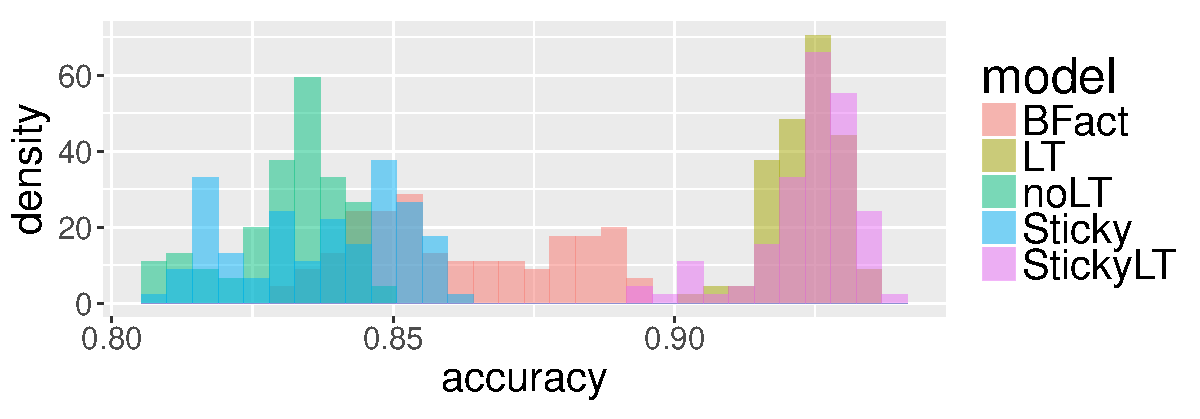
\includegraphics[width = \columnwidth]{fig/cocktail_old/accuracy_density.pdf}}
  \centerline{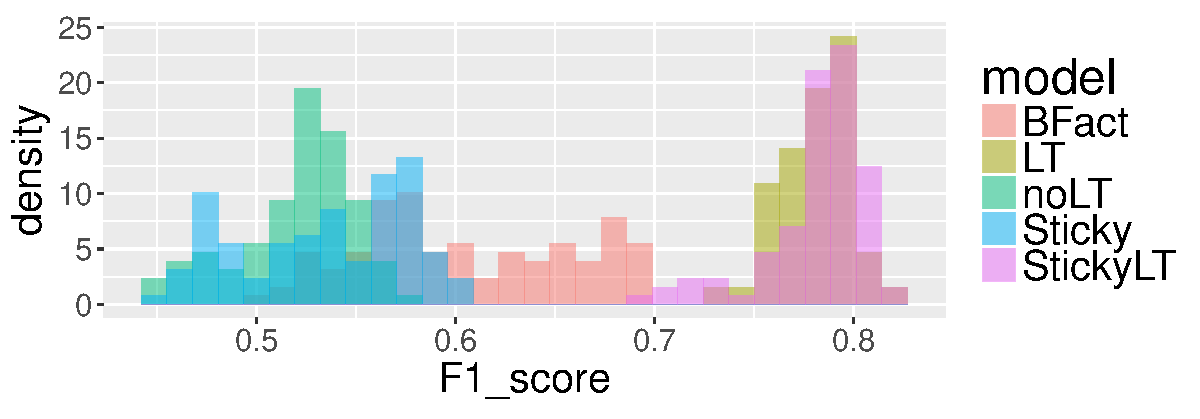
\includegraphics[width = \columnwidth]{fig/cocktail_old/F1_score_density.pdf}}
  \centerline{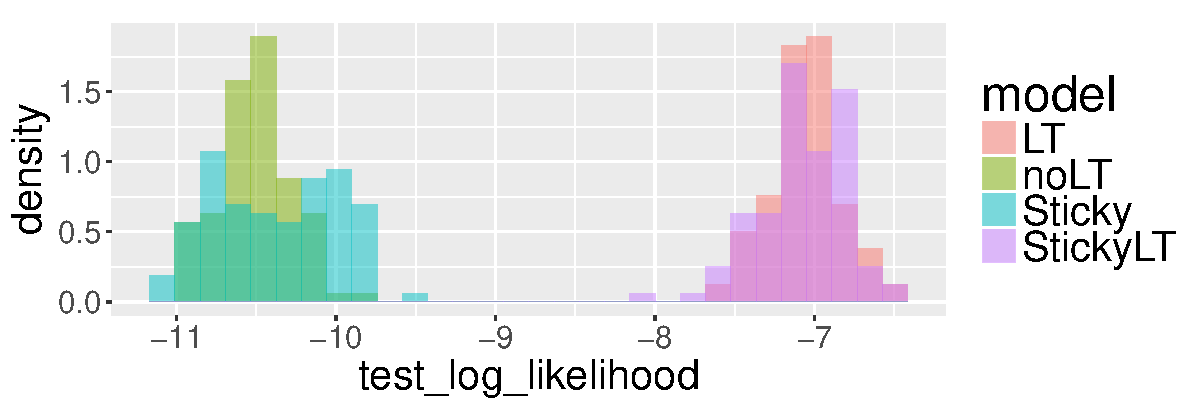
\includegraphics[width = \columnwidth]{fig/cocktail_old/test_log_likelihood_density.pdf}}
  \centerline{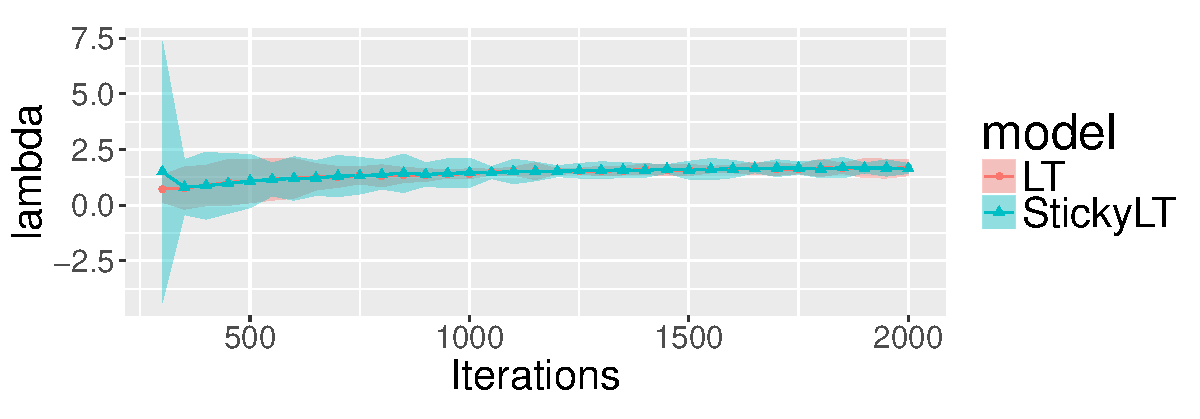
\includegraphics[width = \columnwidth]{fig/cocktail_old/lambda.pdf}}
\caption{(Top) F1 score for inferred relative to ground
  truth binary speaker matrices on cocktail party data, using 
  every 50th Gibbs iteration between 1000-2000, aggregating across 5
  runs of each model. (Middle) Log likelihood on a held out test set.
  (Bottom) Learned similarity parameter, $\lambda$, for the LT and Sticky-LT
  models by Gibbs iteration, averaged over 5 runs.  Error bands are
  99\% confidence interval of the mean.}
\end{center}
\label{fig:cocktail-metrics}
\vskip 0.2in
\end{figure}

\begin{figure}[tb]
\vskip 0.2in
\begin{center}
  \centerline{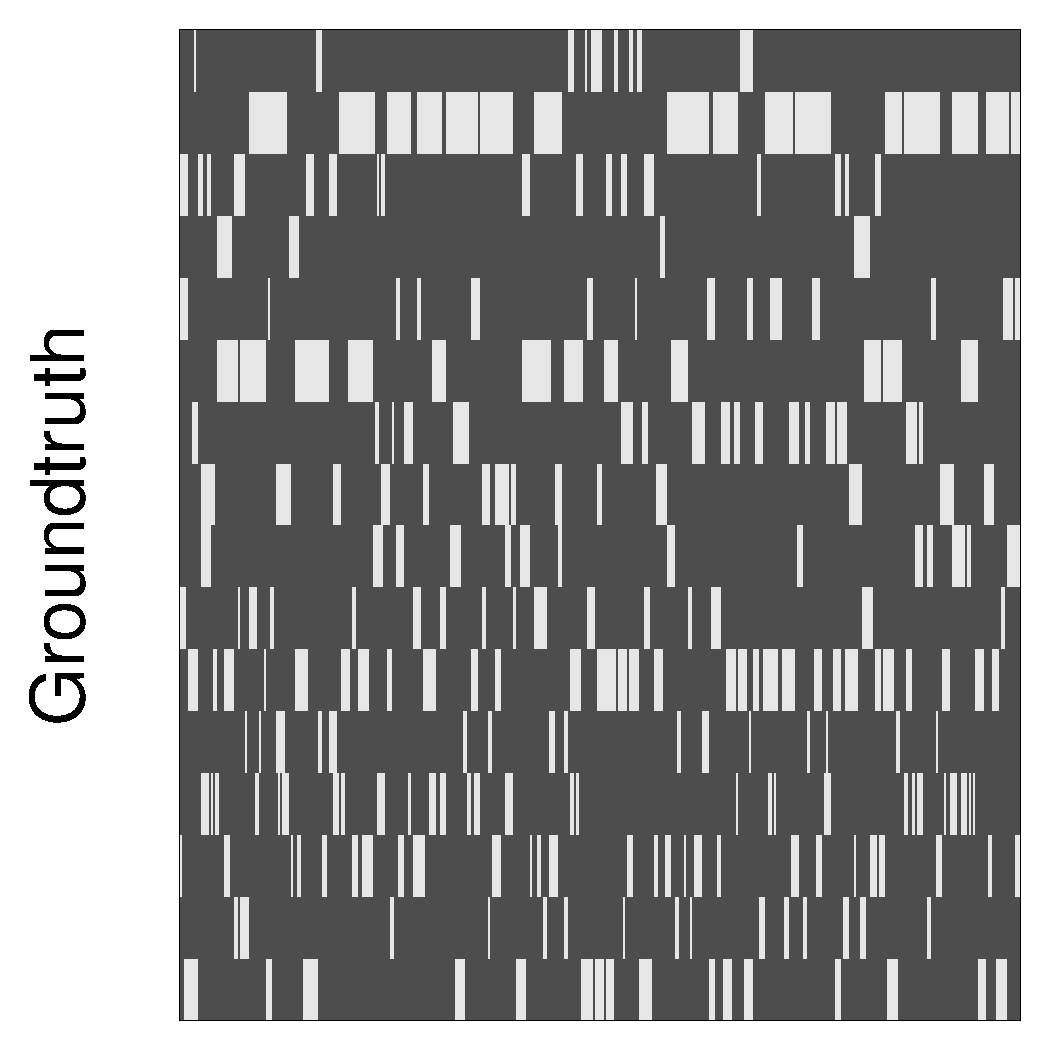
\includegraphics[width = \columnwidth, height = 0.15\columnwidth]{fig/cocktail_old/groundtruth.pdf}}
  \centerline{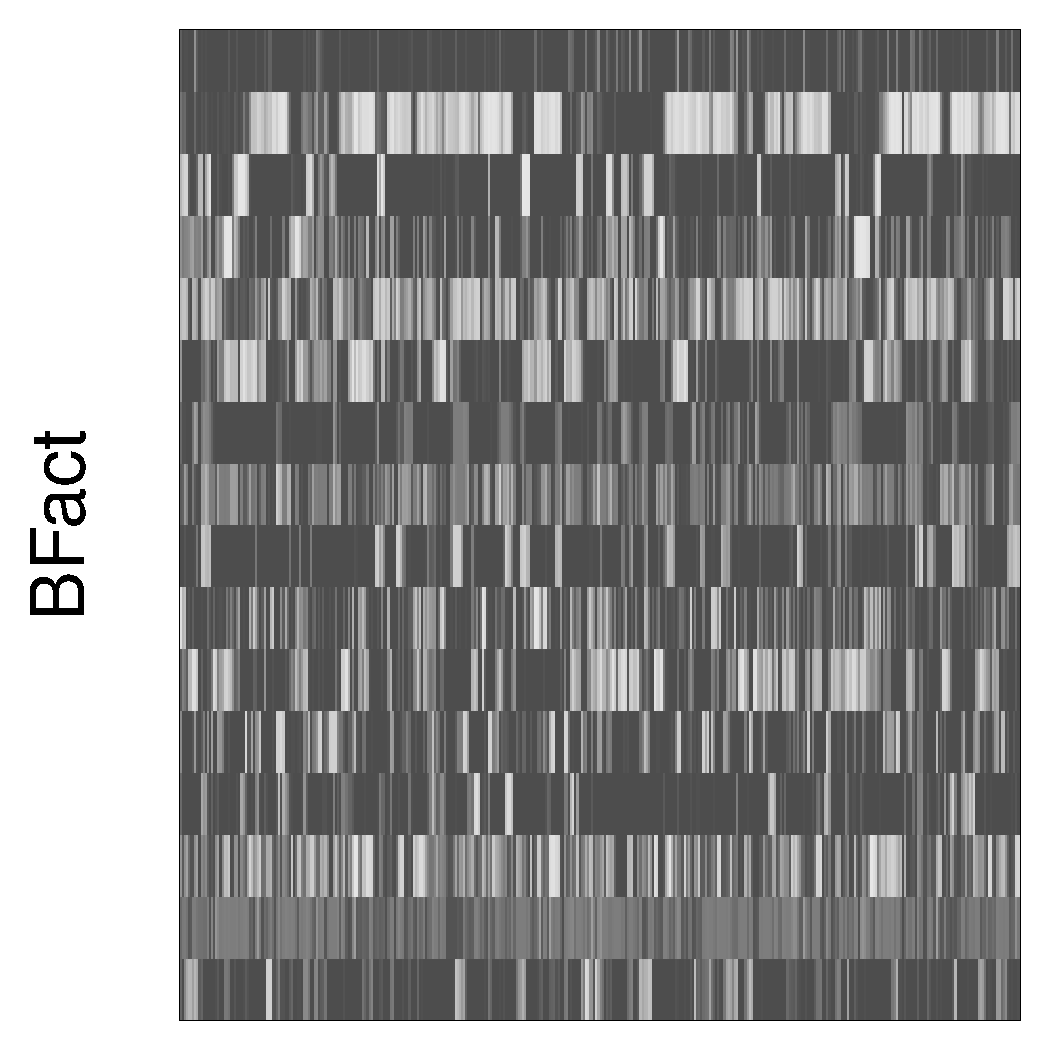
\includegraphics[width = \columnwidth, height = 0.15\columnwidth]{fig/cocktail_old/BFact_hmm_w0_aalpha0p01_balpha0p01/binary_state.pdf}}
  \centerline{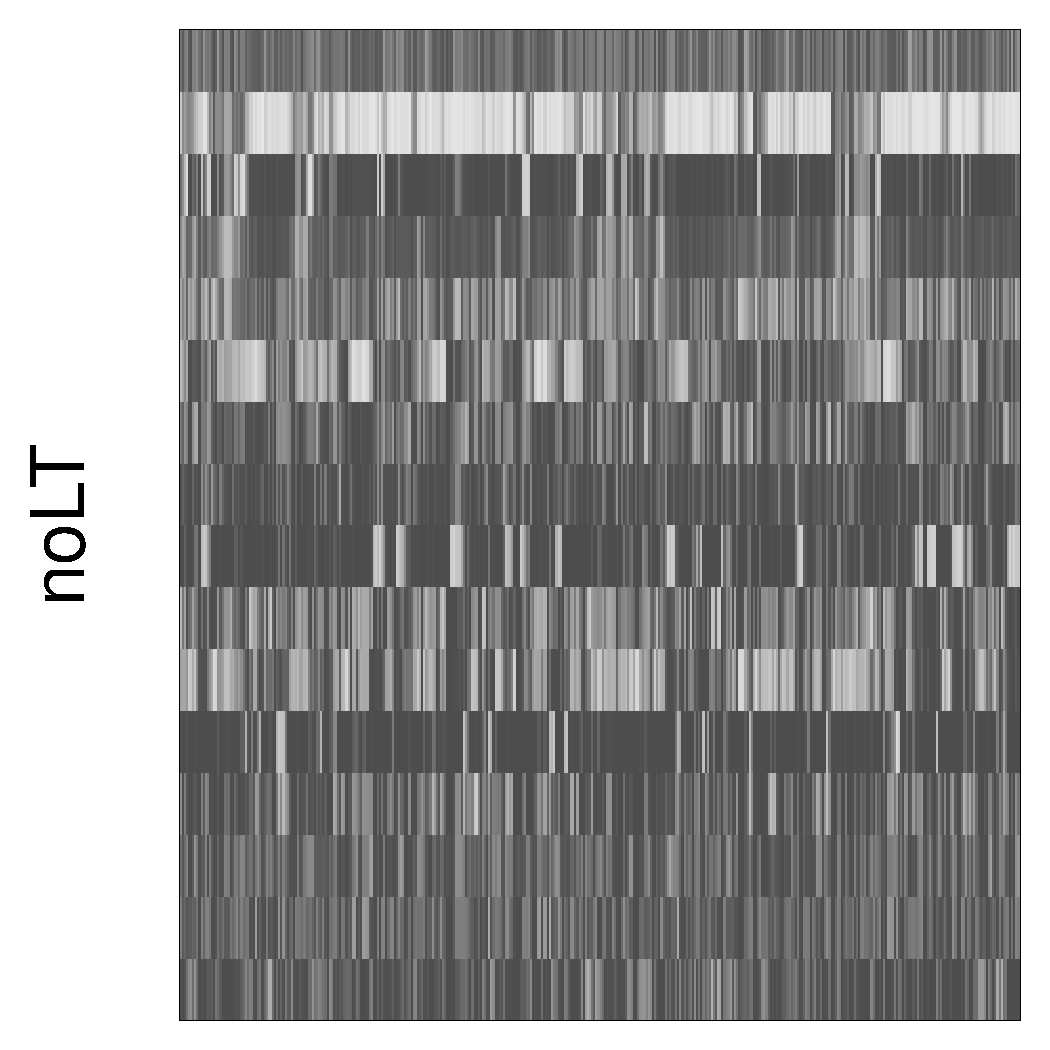
\includegraphics[width = \columnwidth, height = 0.15\columnwidth]{fig/cocktail_old/noLT_hdp_hmm_w0_aalpha0p01_balpha0p01/binary_state.pdf}}
  \centerline{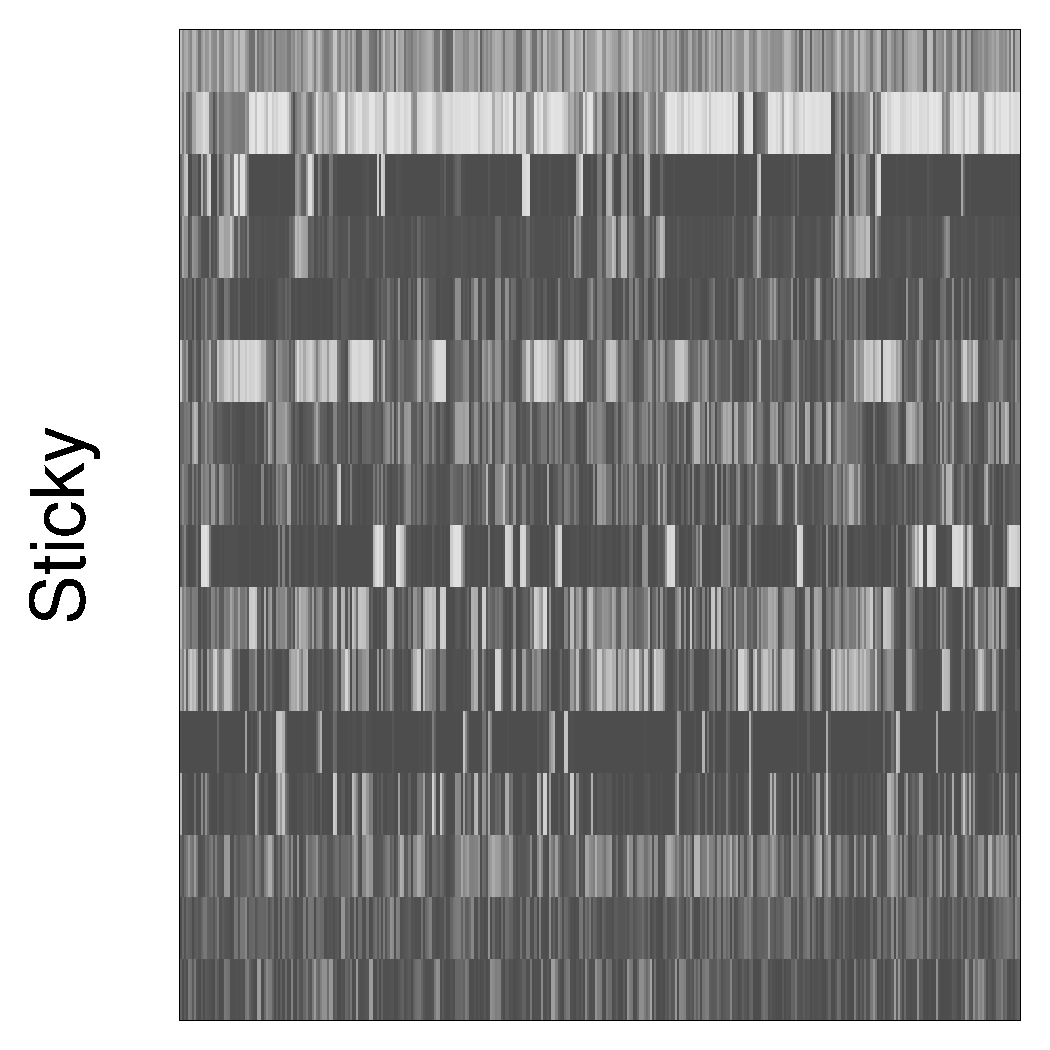
\includegraphics[width = \columnwidth, height = 0.15\columnwidth]{fig/cocktail_old/Sticky_hdp_hmm_w0_aalpha0p01_balpha0p01/binary_state.pdf}}
  \centerline{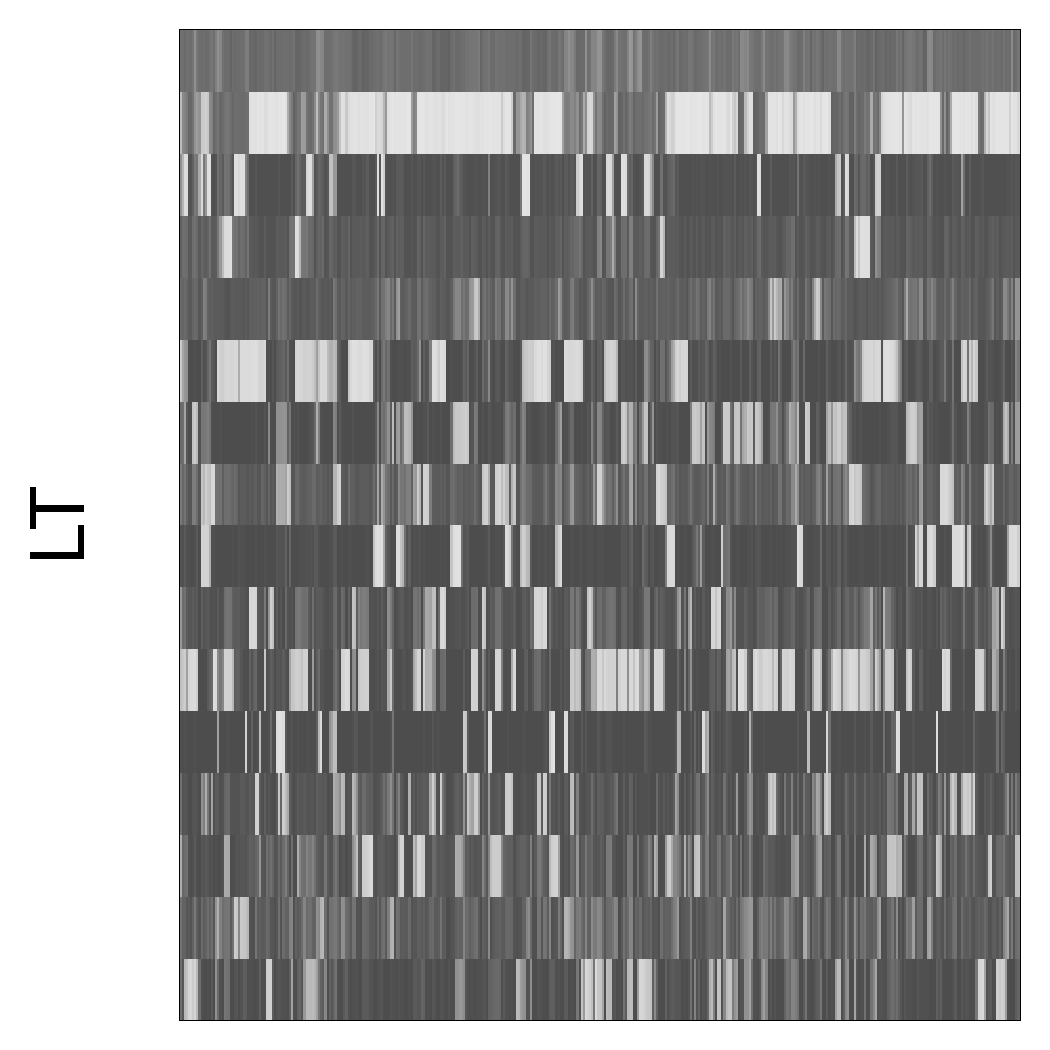
\includegraphics[width = \columnwidth, height = 0.15\columnwidth]{fig/cocktail_old/LT_hdp_hmm_w0_aalpha0p01_balpha0p01/binary_state.pdf}}
  \centerline{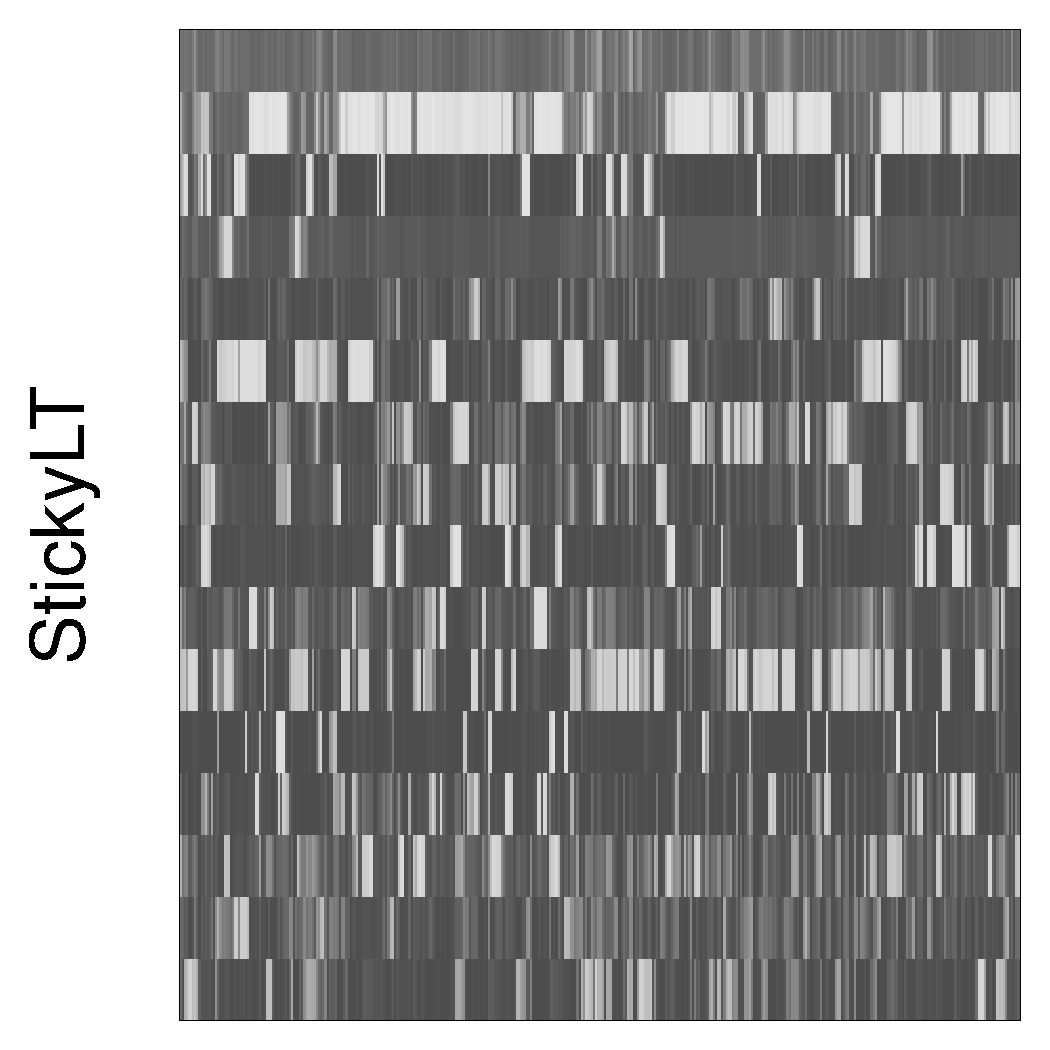
\includegraphics[width = \columnwidth, height = 0.15\columnwidth]{fig/cocktail_old/StickyLT_hdp_hmm_w0_aalpha0p01_balpha0p01/binary_state.pdf}}
\caption{The ground binary speaker matrix for the cocktail party
  data is at the top, followed by the inferred speaker matrix for the
  binary factorial, ``vanilla'' HDP-HMM, Sticky-HDP-HMM, HDP-HMM-LT,
  and Sticky HDP-HMM-LT.  All inferred matrices are averaged over 5 runs and every
  50 iteration after the first 1000.}
\end{center}
\label{fig:cocktail-binary-matrices}
\vskip 0.2in
\end{figure}

\subsection{Synthetic Data Without Local Transitions}
\label{sec:synth-data-without}

We also generated data directly from the ordinary HDP-HMM used in the
cocktail experiment as a sanity check, to examine
the performance of the LT model in the absence of a similarity bias.
The results are in
Fig. \ref{fig:synthetic-metrics}.  When the $\lambda$ parameter is
large, the LT model has worse
performance than the non-LT model on this data;
however, the $\lambda$ parameter settles near zero as the 
model learns that local transitions are not more
probable.  When $\lambda = 0$, the HDP-HMM-LT is an ordinary HDP-HMM.
Unlike on the cocktail party data, the LT model does not use more
states when the data does not have the LT property.

\begin{figure}[tb]
\vskip 0.2in
\begin{center}
  % \centerline{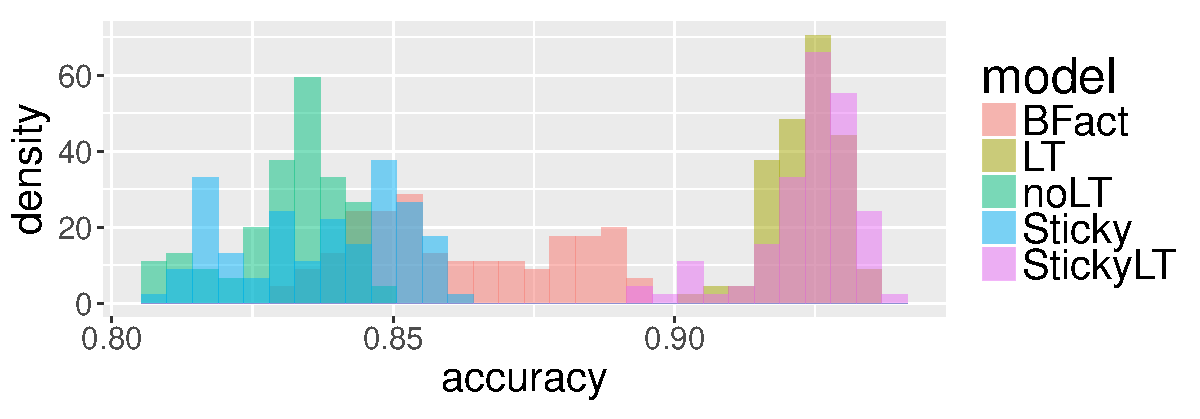
\includegraphics[width = \columnwidth]{fig/cocktail_old/accuracy_density.pdf}}
  \centerline{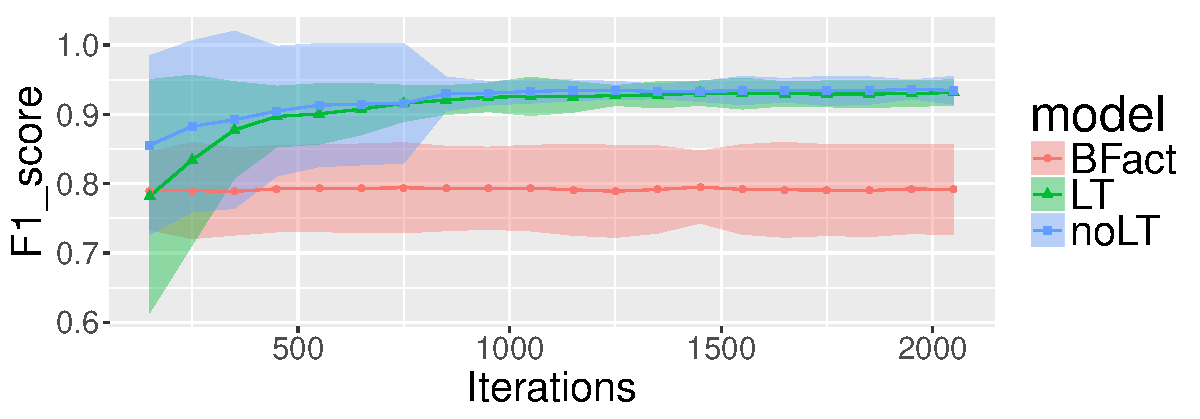
\includegraphics[width = \columnwidth]{fig/synth16/F1_score.pdf}}
  \centerline{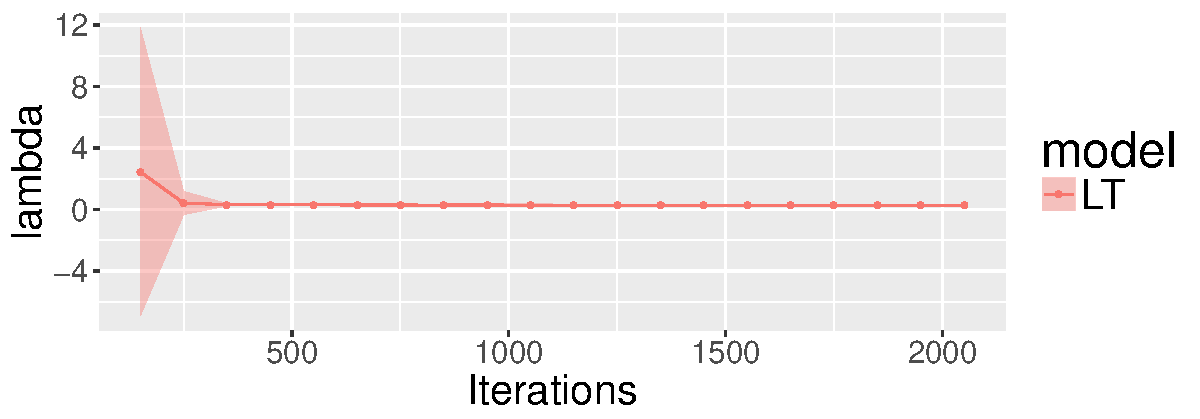
\includegraphics[width = \columnwidth]{fig/synth16/lambda.pdf}}
  \centerline{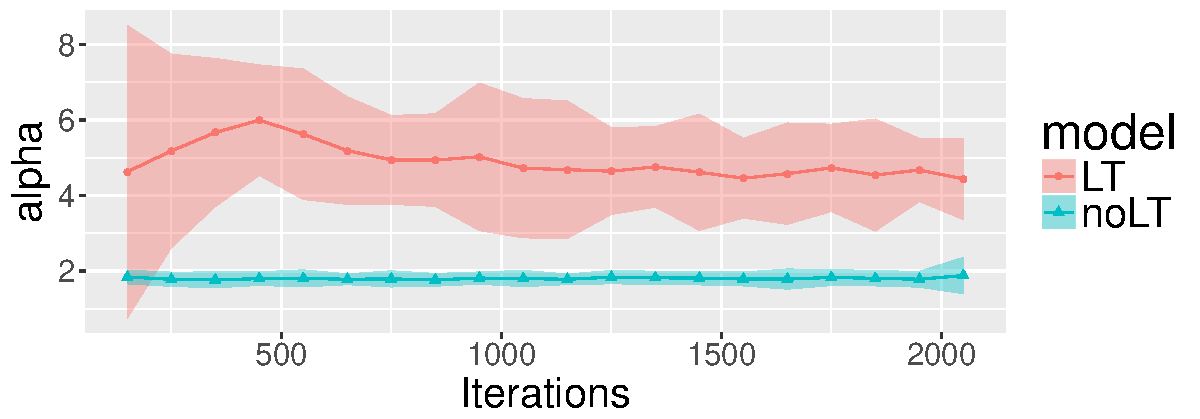
\includegraphics[width = \columnwidth]{fig/synth16/alpha.pdf}}
\caption{(Top) F1 score for inferred relative to ground
  truth binary speaker matrices on synthetic data generated from the
  vanilla HDP-HMM model. (Middle) Learned similarity parameter, $\lambda$, for the LT
  model by Gibbs iteration, averaged over 5 runs.  Error bands are
  99\% confidence interval of the mean.  (Bottom) Concentration
  parameter $\alpha$ for the HDP-HMM-LT and HDP-HMM models.}
\end{center}
\label{fig:synthetic-metrics}
\vskip 0.2in
\end{figure}

% \begin{figure}[tb]
%   \centering
%   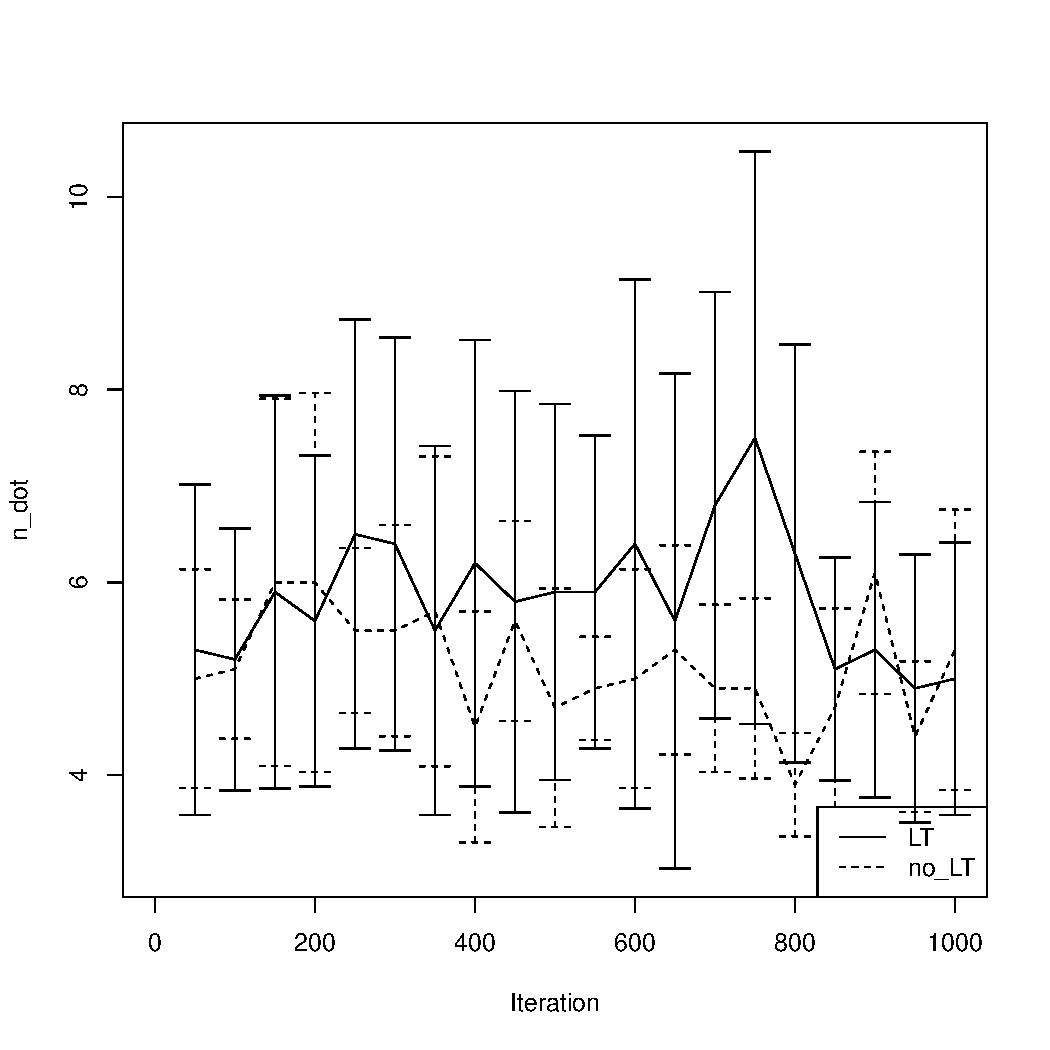
\includegraphics[width = 0.3\textwidth]{fig/synthetic/n_dot}
%   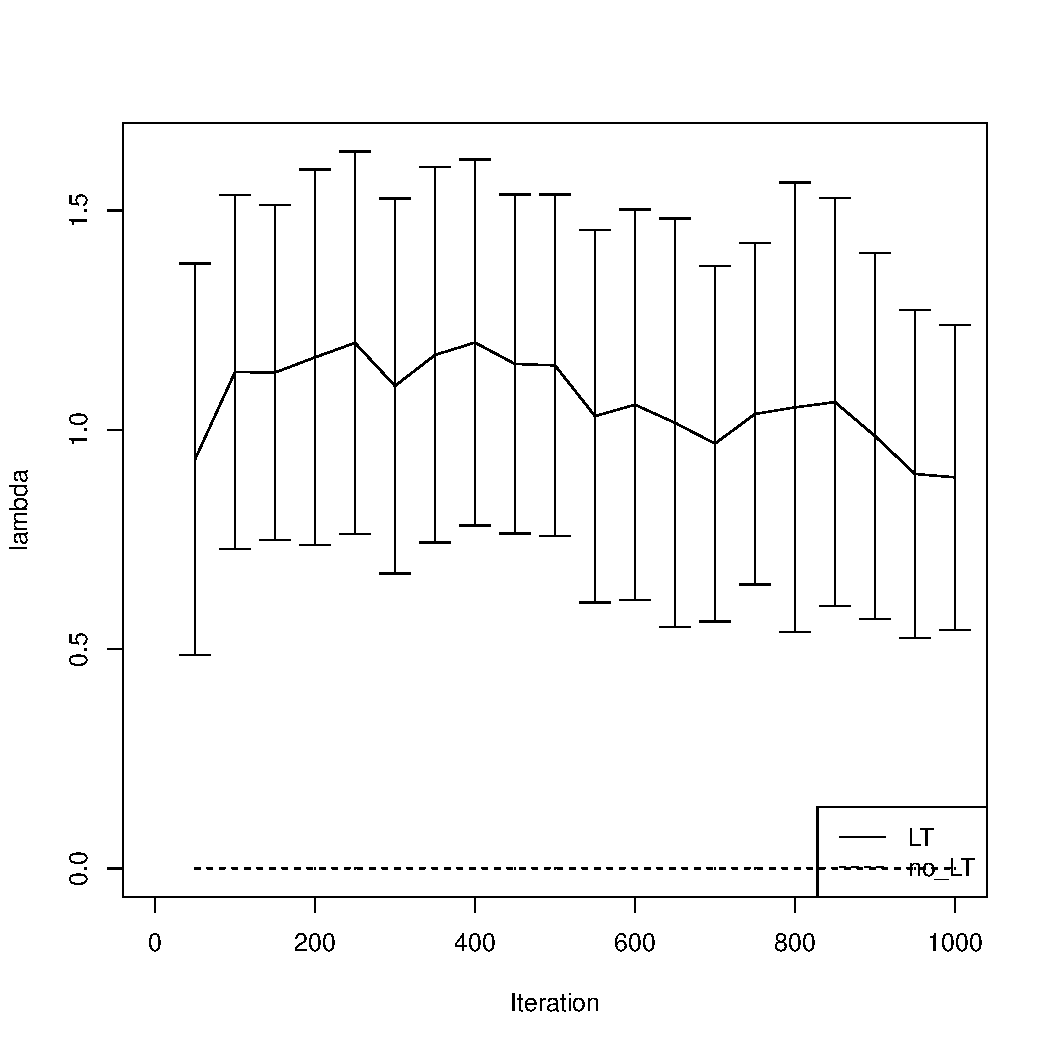
\includegraphics[width = 0.3\textwidth]{fig/synthetic/lambda}
%   \caption{Number of states used on the training data (top), and
%     learned decay rate for the LT model (bottom) on the HDP-HMM data. The first 100
%     iterations are excluded.}
%   \label{fig:synthetic-sparsity}
% \end{figure}

\subsection{Bach Chorales}

To test a version of the HDP-HMM-LT model in which the components of
the latent state governing similarity are unrelated to the emission
distributions, we used our model to do unsupervised ``grammar''
learning from a corpus of Bach chorales.  The data was a corpus of 217 four-voice
major key chorales by J.S. Bach, 200 of which were randomly selected
as a training set, with the other 17 used as a test set to evaluate
surprisal (marginal log likelihood per observation) by the trained
models.  All chorales were transposed to a common key, and each
distinct four-voice chord (with voices ordered) 
was encoded as a single integer.  In total
there were 3307 distinct chord types and 20401 chord tokens in the 217
chorales, with 3165 types and 18818 tokens in the 200 training
chorales, and 143 chord types that were unique to the test set.

Since the chords were encoded as integers, the emission distribution
for each state is $\Cat{\btheta_j}$.  We use a 3307-dimensional 
symmetric Dirichlet prior for each $\btheta_j$, resulting in conjugate 
updates to $\btheta$ conditioned on the latent state sequence, $\bz$.

\paragraph{Modifications to Model and Inference}
\label{sec:model-inference}

In this experiment, the locations, $\bell_j$, are abstract and
independent of the $\btheta_j$.  We use a bivariate
$\Norm{0}{\mathbf{I}}$ prior on each $\bell_j$, and a squared exponential
similarity function based on Euclidean distance: $\phi_{jj} =
\exp\{-\lambda d_2(\bell_j, \bell_{j'})^2\}$ where $d_2$ is Euclidean
distance.  Since the latent
states are now continuous, we use a Hamiltonian Monte Carlo (HMC) update
\cite{duane1987hybrid, neal2011mcmc} to update of the $\bell_j$
simultaneously, conditioned on $\bz$ and $\bpi$.  
HMC is a variation on Metropolis-Hastings
algorithm which is designed to more efficiently explore a
high-dimensional continuous distribution by adopting a proposal
distribution which incorporates an auxiliary ``momentum'' variable to
make it more likely that proposals will go in useful directions and
improve mixing compared to naive movement.  The HMC update requires
the gradient of the log (conditional) posterior.  The relevant prior
and likelihood are
\begin{align}
\begin{split}
  p(\bell_j) &\propto -\frac{1}{2} \norm{\ell_j}^2 \\
  p(\bz, \bu, \bQ \given \bell) &\propto \prod_j \prod_{j'}
  \phi_{jj'}^{n_{jj'}}(1 - \phi_{jj'})^{q_{jj'}}.
\end{split}
\end{align}
The coordinate of the gradient of the log likelihood corresponding to
dimension $d$ in state $j$ is
\begin{equation*}
  \frac{\partial \log L}{\partial \bell_{jd}} = -\lambda
  \sum_{(j,j'):j \neq j'} (\ell_{jd} - \ell_{j'd}) \left(n_{jj'} - q_{jj'} \frac{\phi_{jj'}}{1 - \phi_{jj'}}\right)
\end{equation*}
